\begin{frame}
  \titlepage
\end{frame}

\begin{frame}{Build one widget, understand the whole path}
  \begin{itemize}
    \item Discover and load a custom PHP class.
    \item Declare typed settings and a shared time filter.
    \item Query only the signed-in user's own records.
    \item Return renderer data and choose a safe cache scope.
    \item Verify the contract through PHP, HTTP and the browser.
  \end{itemize}
  \begin{block}{Reference environment}
    MISP 2.5.50, reviewed 29 October 2026. Patch level and theme matter.
  \end{block}
  \note{Allow 35--45 minutes for the presentation and another 25--35 for the
  lab. Learners should know PHP and basic CakePHP conventions. This course
  teaches the integrated dashboard, not the separate ZeroMQ application.
  The README pins the reviewed MISP commit and links to each source contract.
  Do not imply every reviewed feature shipped in the first 2.5 release.}
\end{frame}

\section{Understand the model}

\begin{frame}{A widget extends the integrated dashboard}
  \begin{columns}[T,onlytextwidth]
    \begin{column}{.49\textwidth}
      \begin{block}{The board owns}
        Layout, gallery, configuration, filters, scheduling and export.
      \end{block}
    \end{column}
    \begin{column}{.47\textwidth}
      \begin{block}{Your widget owns}
        Metadata, input validation, data access and renderer-shaped output.
      \end{block}
    \end{column}
  \end{columns}
  \medskip
  Reuse an existing renderer first. Add custom rendering only when the data
  needs a different visual form.
  \note{The dashboard is inside MISP at /dashboards. No standalone subscriber
  or Flask service is involved. Explain that a widget is a PHP class, not a
  new board framework. The modern board supplies typed configuration,
  accessible controls and scheduling. Keep external dependencies out of the
  first exercise so data boundaries are easy to inspect.}
\end{frame}

\begin{frame}{The render request has a defined pipeline}
  \centering
  \begin{tikzpicture}[
    node distance=.40cm,
    stage/.style={draw=mispTeal,rounded corners,fill=mispBlue!5,
      text width=8.0cm,align=center,minimum height=.62cm,font=\small},
    flow/.style={-{Stealth},thick,draw=mispTeal}]
    \node[stage] (load) {Load class and check permissions};
    \node[stage,below=of load] (adapt) {Inject missing defaults; adapt canonical config};
    \node[stage,below=of adapt] (cache) {Cache hit, or call handler with authenticated user};
    \node[stage,below=of cache] (render) {Select renderer; return HTML or REST payload};
    \draw[flow] (load)--(adapt);
    \draw[flow] (adapt)--(cache);
    \draw[flow] (cache)--(render);
  \end{tikzpicture}
  \sources{Source: DashboardsController::renderWidget}
  \note{CanonicalTypeAdapter runs before WidgetCache. A cache hit does not
  execute handler validation or its query; keep cached output valid for the
  entire cache audience. Permission checks still happen before the cache.
  The normal web request uses the HTML renderer; JSON callers receive an
  envelope. The full PHP example follows this pipeline without implementing
  its own adapter or cache.}
\end{frame}

\begin{frame}[fragile]{Discovery: filename, class and location}
\begin{lstlisting}
app/Lib/Dashboard/Custom/
  TrainingLoginSummaryWidget.php

class TrainingLoginSummaryWidget
{
    // Metadata and handler live here.
}
\end{lstlisting}
  \begin{itemize}
    \item Use a unique class ending in \code{Widget}.
    \item Match the filename exactly; no registration list.
    \item Built-in classes take precedence over Custom.
  \end{itemize}
  \note{Dashboard::loadAllWidgets scans built-ins, Custom and one level of
  custom subdirectories for files ending Widget.php. The loader looks for
  the built-in class path first. WhoamiWidget already exists, so the new
  exercise deliberately avoids overriding it. A missing or disallowed class
  is not a renderer problem. Inspect PHP syntax, worker read permissions
  and class discovery before debugging the UI.}
\end{frame}

\begin{frame}{Metadata gives the gallery a useful entry}
  \small
  \begin{tabular}{P{.30\textwidth}P{.61\textwidth}}
    \toprule
    Property & Purpose \\
    \midrule
    \code{title}, \code{description} & Explain the result and its data scope. \\
    \code{category}, \code{thumbnail} & Help discovery; thumbnail is optional. \\
    \code{render} & Name an existing renderer, here \code{SimpleList}. \\
    \code{width}, \code{height} & Initial tile dimensions. \\
    \code{schema} & Typed configuration and canonical filter declarations. \\
    \code{params}, \code{placeholder} & Advanced option documentation and example JSON. \\
    \bottomrule
  \end{tabular}
  \note{These are public PHP properties. This example declares no thumbnail
  and relies on the renderer preview. The gallery endpoint enriches the
  older metadata extraction with schema, category and thumbnail. Placeholder
  content is not a default policy or an access check. A dynamic renderer may
  implement getRenderer(config); ensure all its possible data shapes match.}
\end{frame}

\begin{frame}{Two decisions: who may load it, what may they read?}
  \begin{block}{Widget permission}
    \code{checkPermissions($user)} gates discovery and loading.
  \end{block}
  \begin{block}{Data permission}
    The handler must apply the right user, organisation or event-access scope
    to its query.
  \end{block}
  \medskip
  A visible gallery card does not make every database row visible.
  \note{The example accepts an authenticated positive numeric user ID. The
  handler repeats the identity check for direct invocation, but trusts only
  the user supplied by the framework. A caller-supplied config.user\_id is
  rejected. For event data, use the relevant ACL-aware MISP retrieval API:
  arbitrary model find calls are not automatically access-scoped. Some
  built-in aggregate widgets intentionally report global counts; their
  semantics cannot be copied blindly to a detailed personal widget.}
\end{frame}

\section{Build the example}

\begin{frame}{Our exercise: my sign-in history}
  \screenshot{images/training-widget.png}
  \note{This is a genuine default-theme browser capture from the reviewed
  2.5.50 source. The account is an ordinary User in a synthetic organisation.
  Its login audit timestamp was created by a real browser login in the lab.
  The widget shows user ID and sign-in times, not emails, IPs or another
  user's data. This is a bounded teaching exercise; it is not a proposal to
  duplicate the existing core Whoami widget.}
\end{frame}

\begin{frame}[fragile]{Declare the canonical time-window setting}
\begin{lstlisting}[language=PHP]
public $schema = [
    'lookback' => [
        'type' => 'time_window',
        'default' => 'P7D',
        'help' => 'Your own sign-ins; at most 366 days.',
    ],
    // Scalar fields follow in the complete example.
];
\end{lstlisting}
  The shared toolbar follows the declared \textbf{type}, not the name
  \code{lookback}.
  \note{This abbreviated schema excerpt keeps the contract visible on screen.
  The complete file has a fuller help string. The canonical declaration
  enables the typed configuration control and toolbar reachability. Choosing
  a parameter name such as lookback is valid; time\_window does not have to be
  the key name. Do not declare a canonical type unless the handler can
  consume its adapter output.}
\end{frame}

\begin{frame}{Canonical inputs and scalar settings serve different jobs}
  \begin{block}{Shared concepts}
    Time, tags, organisations, sharing groups, galaxy clusters,
    distribution, threat level and analysis state.
  \end{block}
  \begin{block}{Widget-specific settings}
    \code{string}, \code{int}, \code{bool}, \code{enum}.
    Here: caption, result limit and organisation checkbox.
  \end{block}
  \medskip
  \code{attribute_type_filter} and \code{event_id_filter} are canonical,
  but are not toolbar controls in this snapshot.
  \note{WidgetSchema defines twelve canonical types, ten of which are toolbar
  eligible. The README lists all names, including org\_meta\_filter and
  date\_range. Scalar types do not create toolbar chips. Enum declarations
  require an enum list and can provide enum\_labels. A shared toolbar change
  affects only widgets that declare the relevant canonical type. Avoid
  inventing universal tag-filter syntax: widget contracts still differ.}
\end{frame}

\begin{frame}{The adapter changes what the handler receives}
  \begin{center}
  \begin{tabular}{ll}
    \toprule
    Saved / wire value & Handler value \\
    \midrule
    \code{P7D} & \code{7d} \\
    \code{P2W} & \code{14d} \\
    \code{PT6H} & \code{21600} seconds \\
    \code{-1} & All-time sentinel, unchanged \\
    \bottomrule
  \end{tabular}
  \end{center}
  \begin{alertblock}{Defaults do not mean validation}
    Missing keys get defaults. Explicit nulls, empty strings and unknown
    shapes may reach your handler.
  \end{alertblock}
  \note{The verifier invokes the real CanonicalTypeAdapter before the
  example handler. Legacy day strings and raw seconds are preserved.
  The adapter is deliberately compatibility-oriented, so validate its
  resulting values. This example accepts positive seconds up to 366 days,
  bounded day strings and minus one; rejects zero, booleans, null, arrays,
  oversized windows and unknown strings. Other canonical types have their
  own translations and validation; inspect those before adopting them.}
\end{frame}

\begin{frame}{Typed configuration, visible in the real panel}
  \begin{columns}[c,onlytextwidth]
    \begin{column}{.54\textwidth}
      \centering
      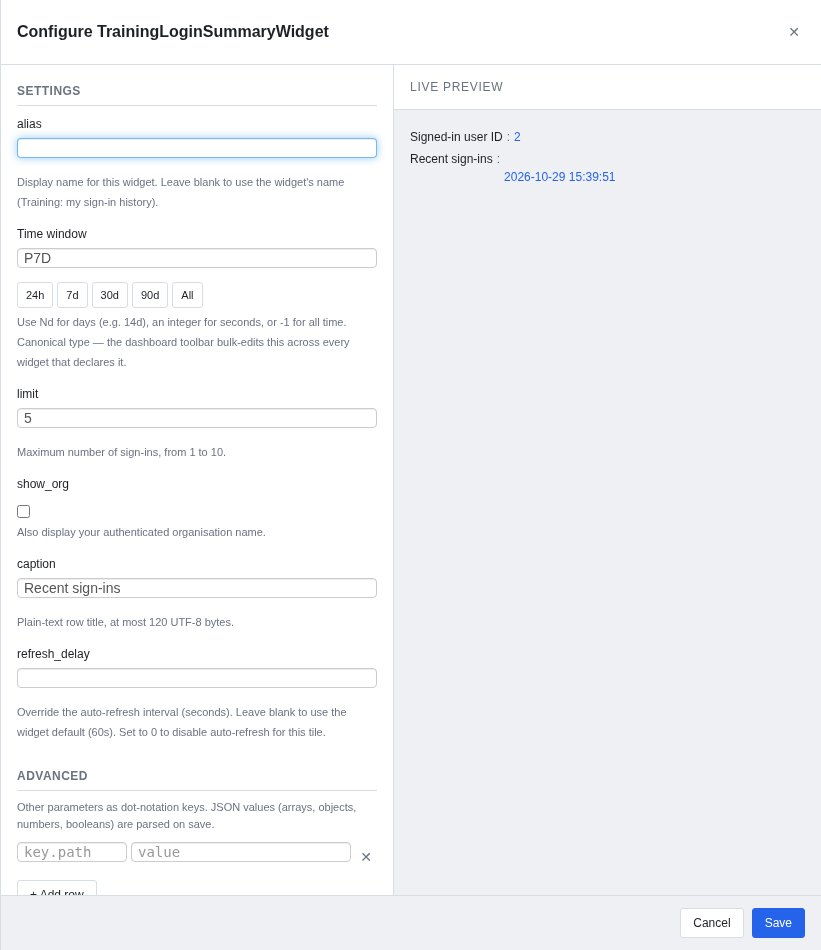
\includegraphics[height=6.0cm,width=\textwidth,keepaspectratio]{images/typed-configuration.png}
    \end{column}
    \begin{column}{.42\textwidth}
      \begin{itemize}
        \item Time-window control.
        \item Integer result limit.
        \item Boolean checkbox.
        \item Plain-text caption.
      \end{itemize}
      \small The panel saves configuration separately from layout editing.
    \end{column}
  \end{columns}
  \note{Use a live demonstration or the larger README image to inspect the
  field labels. The capture includes framework-managed alias and
  refresh\_delay fields and an advanced section. They are not extra SQL
  parameters. The browser test changed the caption to HTML-like text,
  enabled the checkbox, saved successfully and confirmed literal rendering.
  Do not present a screenshot alone as proof of persistence or validation.}
\end{frame}

\begin{frame}{Validate before querying}
  \begin{itemize}
    \item \code{limit}: integer from 1 to 10.
    \item \code{show_org}: real boolean, not the string \code{"false"}.
    \item \code{caption}: nonempty UTF-8, at most 120 bytes, no controls.
    \item Reject unknown keys, including a supplied \code{user_id}.
  \end{itemize}
  \begin{block}{Framework-owned settings}
    Accept \code{alias} and \code{refresh_delay}; do not let them change data.
  \end{block}
  \note{BadRequestException yields HTTP 400 for these handler failures in the
  live test. Do not cast strings to booleans: the nonempty string false is
  truthy in PHP. The example uses strict is\_int and is\_bool checks and
  array\_key\_exists so explicit null does not silently become a default.
  This is one possible public contract; compatible existing widgets may
  need a documented migration path instead of immediate strict rejection.}
\end{frame}

\begin{frame}[fragile]{Apply identity in the actual SQL conditions}
\begin{lstlisting}[language=PHP]
$conditions = [
    'Log.user_id' => (int)$user['id'],
    'Log.action' => 'login',
];
if ($seconds !== -1) {
    $conditions['Log.created >='] =
        date('Y-m-d H:i:s', time() - $seconds);
}
\end{lstlisting}
  Query identity comes from the authenticated user, never configuration.
  \note{This is the data boundary. Date formatting follows Log::beforeSave's
  use of date in the application's PHP timezone. The handler also bounds
  output with a selected field list, recursive minus one and limit 1--10.
  Ordering is created descending and then ID descending for stable ties.
  A limit caps returned rows; it is not proof that a query is inexpensive.
  For larger audit tables, inspect query plans and indexes rather than
  adding broad unbounded scans to frequently refreshed widgets.}
\end{frame}

\begin{frame}[fragile]{Return the renderer's data, not a page}
\begin{lstlisting}[language=PHP]
$rows = [
    ['title' => 'Signed-in user ID',
     'value' => (string)$user['id']],
    ['title' => $caption,
     'value' => $times ?: 'No matching sign-ins.'],
];
return $rows;
\end{lstlisting}
  \code{SimpleList} accepts scalar or array values.

  Empty history is a valid result. A database failure is an error.
  \note{The snippet omits the optional organisation row for readability.
  The real template escapes title and value and joins array values with
  line breaks. The example returns plain timestamps, not HTML. It deliberately
  does not catch database exceptions and return an empty array, because that
  would hide a failure as no activity. Test empty data and backend failure
  independently.}
\end{frame}

\begin{frame}{Escaping belongs at the output sink}
  \begin{block}{Use plain values}
    \code{<b>Plain text</b>} should appear as text in the widget.
  \end{block}
  \begin{itemize}
    \item \code{SimpleList} escapes \code{title} and \code{value}.
    \item \code{html} and \code{html_title} deliberately bypass escaping.
    \item \code{drilldown} is checked by the dashboard URL validator.
  \end{itemize}
  \note{Do not pre-escape text, which causes double escaping in the real
  renderer. Avoid raw HTML fields for user-controlled content. URL validation
  drops dangerous schemes and arbitrary off-host URLs; permitted origins
  include the MISP origin and the configured CVE reference origin. Test the
  actual PHP element as well as JSON. The committed verifier includes the
  real SimpleList template with actual CakePHP h() rather than reproducing
  its rendering logic in a fake helper.}
\end{frame}

\begin{frame}{Refresh interval and cache TTL are different}
  \small
  \begin{center}
    \begin{tabular}{ll}
      \toprule
      Example property & Meaning \\
      \midrule
      \code{autoRefreshDelay = 60} & Request a refresh every 60 seconds \\
      \code{cache_duration = 30} & Reuse a result for 30 seconds \\
      \code{cache_scope = 'user'} & Separate cached results by user \\
      \bottomrule
    \end{tabular}
  \end{center}
  \medskip
  Manual refresh can return a cache hit. Redis failure falls back to live work.
  \note{These are public properties with dollar prefixes in PHP. The
  legacy cacheLifetime property taught in the earlier lesson does not opt
  into the generic cache in this reviewed controller. Positive cache\_duration
  enables it; zero disables it. An optional cache\_path changes the prefix.
  The default prefix is derived from the class name. During debugging,
  use a disabled cache or wait for expiry before drawing conclusions about
  code changes; do not recommend flushing a shared Redis database.}
\end{frame}

\begin{frame}{Choose cache scope from the output's audience}
  \small
  \begin{tabular}{P{.17\textwidth}P{.72\textwidth}}
    \toprule
    Scope & Appropriate when \\
    \midrule
    Default & The same config yields identical data for every viewer. \\
    \code{org} & An aggregate is identical within an organisation; site admins
      have a separate unrestricted bucket. \\
    \code{user} & Personal identity, role or access changes the result. \\
    \bottomrule
  \end{tabular}
  \begin{alertblock}{This example needs user scope}
    Two users in the same organisation have different sign-in histories.
  \end{alertblock}
  \note{A private SQL query followed by a shared cache can still leak data.
  Permissions and cache audience are separate decisions. WidgetCache keys
  the translated config, sorted at top level, and excludes alias and
  refresh\_delay. Thus the handler must not make its data depend on those
  fields. The verifier checks real helper keys for same-org users;
  the integration test exercises A/B/A through actual HTTP and Redis.
  Missing usable identity causes scoped remember to run live rather than
  cache in a shared bucket.}
\end{frame}

\section{Verify and contribute}

\begin{frame}[fragile]{Test the wrapped REST contract}
\lstinputlisting[language=json]{examples/render-request.json}
  \code{POST /dashboards/renderWidget}
  \begin{itemize}
    \item Response: widget, instance ID, translated config, renderer, data.
    \item \code{/exportjson:1}: bare handler data.
    \item \code{/exportcsv:1}: flattened CSV.
  \end{itemize}
  \note{The README gives a curl command with a locally provided API key,
  JSON content type and Accept header. Never commit a real key or turn off
  TLS validation. The controller accepts config as an object or JSON string;
  teach the object form. The response config uses 7d after adaptation, unlike
  the saved canonical P7D. A successful REST payload proves neither safe
  HTML rendering nor a functioning JavaScript chart. Keep normal CSRF
  handling in browser requests.}
\end{frame}

\begin{frame}[fragile]{A layout identifies instances, not just classes}
\begin{lstlisting}[language=json]
[
  {
    "instance_id": "training_signins",
    "widget": "TrainingLoginSummaryWidget",
    "config": {"lookback": "P7D", "limit": 5},
    "position": {"x": 0, "y": 0, "w": 6, "h": 4}
  }
]
\end{lstlisting}
  Keep instance IDs stable. Importing a layout changes the personal board.
  \note{This shortened illustration omits optional example config keys;
  schema defaults supply them. The complete importable layout is in examples.
  Multiple instances of a class can have different IDs and settings.
  Older width/height-only layouts have adaptation paths, but new examples
  should use position x/y/w/h. GET /dashboards returns the REST layout;
  /dashboards/export instead wraps saved UserSetting data. Import and
  template selection never grant access to underlying records.}
\end{frame}

\begin{frame}{Saving layout does not save every kind of change}
  \begin{block}{Layout staging}
    Add, move, resize and remove; then Save changes or Discard.
  \end{block}
  \begin{block}{Configuration persistence}
    The configure panel and shared toolbar save settings separately.
  \end{block}
  \medskip
  A layout Discard is not a universal undo.
  \note{Controller updateSettings saves the personal UserSetting dashboard
  layout. updateWidgetSettings patches configurations separately. Shared
  templates are Dashboard records. Learners should export a board before
  experimenting, and save settings, reload and inspect server state rather
  than assuming an in-memory preview means persistence. This separation
  also matters when writing integration tests.}
\end{frame}

\begin{frame}{Three layers of evidence}
  \small
  \begin{tabular}{P{.22\textwidth}P{.67\textwidth}}
    \toprule
    Layer & Verify \\
    \midrule
    PHP contracts & Real schema, adapter, cache keys and template;
      recorded database boundary. \\
    Live HTTP & Actual SQL results, user A/B/A, invalid inputs, export and
      layout import/readback. \\
    Browser & Discovery, typed settings, saved state, literal caption,
      resize and usable controls. \\
    \bottomrule
  \end{tabular}
  \medskip
  The supplied verifier runs \textbf{59 checks}; it is not an integration test.
  \note{The standalone verifier loads actual CakePHP helpers and MISP
  classes from a provided installation. Only Log::find is replaced with an
  in-memory recorder; it tests query arguments and failure propagation.
  It does not access SQL, Redis or HTTP. The real lab separately verified
  two non-admin users in the same org, genuine logins, rejection cases,
  wrapped/bare JSON, import/readback and browser config saves. Be precise
  about evidence rather than describing a mock query as a tested database.}
\end{frame}

\begin{frame}{Workshop: install, challenge, remove}
  \begin{enumerate}
    \item Export your board; install the one custom PHP file.
    \item Lint it and run \code{verify_widget.php} against MISP.
    \item Add the widget; save a caption and checkbox setting.
    \item Render as A, B, A within the cache TTL.
    \item Try an invalid boolean, limit, null and supplied user ID.
    \item Restore the board and remove the training PHP file.
  \end{enumerate}
  \note{Use two disposable ordinary users in the same organisation and
  sign in through the browser to generate Log.action login rows.
  The README includes exact installation and request commands. An API key
  requires API permission but no site-admin role for this widget. Installation
  requires operator access to the custom directory. Check permissions if the
  gallery entry is absent. Removing a class while leaving its instance in a
  board creates a missing-widget state, so clean the layout first.}
\end{frame}

\begin{frame}{Port the older lesson deliberately}
  \small
  \begin{tabular}{P{.38\textwidth}P{.52\textwidth}}
    \toprule
    Earlier pattern & Reviewed 2.5 model \\
    \midrule
    Name collision / mismatched file & Unique matching class and filename \\
    \code{params} only & Schema plus deliberate legacy support \\
    \code{cacheLifetime} & Duration and appropriate cache scope \\
    Renderer assumptions & Actual element and data contract \\
    Size-only layout & Stable IDs and position coordinates \\
    Ad hoc testing & Contracts, live requests and browser checks \\
    \bottomrule
  \end{tabular}
  \note{The original lesson, assets and PDF are preserved in the archive and
  excluded from standard training. Migrate saved configs intentionally:
  adding a schema does not rewrite them or secure an old query. Preserve
  compatibility where it matters and document deliberate changes. Cache
  invalidation after changing output semantics needs an operator plan;
  a temporary cache disable or new dedicated prefix is safer than a broad
  shared-cache flush.}
\end{frame}

\begin{frame}{If a new renderer is necessary}
  \begin{itemize}
    \item Start with the PHP element's precise data shape.
    \item Reuse theme tokens and accessible, responsive markup.
    \item Extend the existing dashboard chart modules where needed.
    \item Add a gallery preview for the renderer.
    \item Test empty data, failures, resizing, keyboard and themes.
  \end{itemize}
  \note{PHP renderer elements are in app/View/Elements/dashboard/Widgets.
  JavaScript lives under app/webroot/js/dashboard, with chart modules under
  charts and preview glyph handling at gallery/render-thumbs.mjs.
  Reuse the deployed assets and framework instead of dropping in replacement
  vendor libraries or inline scripts. For SimpleList no JavaScript renderer
  is needed. A new renderer should come with evidence that HTML and chart
  initialization work, not just a screenshot of JSON.}
\end{frame}

\begin{frame}{Make the contribution reviewable}
  \begin{itemize}
    \item State the question the widget answers and the audience.
    \item Document schema, data visibility, refresh and cache scope.
    \item Include focused checks and a reproducible lab procedure.
    \item Show real UI evidence with synthetic data.
    \item Explain saved-config compatibility and deployment needs.
  \end{itemize}
  \begin{block}{Continue from the repository}
    Working example, request, layout, verifier and pinned source audit
    are in \code{a.a-widget-dev/README.md}.
  \end{block}
  \note{Review MISP's current contribution guidance before proposing a core
  widget. Custom deployments can keep a local class without upstreaming it.
  This example intentionally duplicates a simple personal-status concept
  for teaching, so do not submit it as a new core feature unchanged.
  Reviewers should be able to reproduce data-boundary and cache-isolation
  checks without a production dataset or a committed credential.}
\end{frame}
